\documentclass[12pt,a4paper]{article}
\usepackage[francais]{babel}
\usepackage[utf8x]{inputenc} 
\usepackage[T1]{fontenc}
\usepackage{dsfont}
\usepackage{ucs}
\usepackage[pdftex]{graphicx}
\usepackage{amsmath}
\usepackage{amsfonts}
\usepackage{amssymb}
\title{Notes de cours de CRYPTOLOGIE}
\author{rédigées par Julien Audebert et Lionel Rivière}
\begin{document}

\maketitle

\tableofcontents

\newpage 

%%%%%%%%%%%%%%%%%%%%%%%%%%%%%%%%%%%%%%%%%%%%%%%%%%%%%%%%%
%             		Julien AUDEBERT                     %
%%%%%%%%%%%%%%%%%%%%%%%%%%%%%%%%%%%%%%%%%%%%%%%%%%%%%%%%%
\section{Introduction}

Les besoins de la cryptologie:
\begin{itemize}
\item Confidentialité (Secret)
\item Intégrité (des messages)
\item Authentification (émetteur, destinataire)
\item Non-répudiation
\end{itemize}

Quelques exemples d'utilisation:
\begin{itemize}
\item Paiement
\item Monnaie numérique
\item vote électronique
\item ventes aux enchères
\item Pour garder l'ANONYMAT
\end{itemize}

\subsection{Chiffrement}

\begin{center}
Modèle Standard
\begin{displaymath}
A,M \stackrel{C=f(M)}{\longrightarrow} B M=f^{-1}(C)
\end{displaymath}
O
\end{center}

\begin{itemize}
\item A émetteur \textbf{chiffre}
\item B récepteur \textbf{déchiffre}
\item O observateur (passif) \textbf{décrypte}
\item M message en clair
\item C message chiffré (cryptogramme)
\item f transformation secrète de chiffrement
\end{itemize}

Le secret est partagé entre A et B.

\subsection{Système de Chiffrement (Chiffre)}
$(f_k)_{k \in \mathbb{K}}$  $K$ est l'ensemble des <<clés>>.

$(f_k)$ définit l'ensemble des fonctions permettant de chiffrer

\subsubsection{Chiffrement de César}
\begin{displaymath}
A\longrightarrow D
\end{displaymath}
\begin{displaymath}
B\longrightarrow E
\end{displaymath}
\begin{displaymath}
C\longrightarrow F
\end{displaymath}

\subsubsection{Chiffrement par substitution}

$(f_{\sigma})$ où $\sigma$  est une permutation de l'ensemble $\{A,B,C,....,Z\}$

\bigskip

CRYPTO $\to f(CRYPTO)=\sigma(C)|\sigma(R)|\sigma(Y)|\sigma(P)|\sigma(T)|\sigma(O)$

\subsubsection{Chiffrement par permutation (transposition)}

\begin{displaymath}
\begin{array}{cccccc}
1 & 2 & 3 & 4 & 5 & 6 \\
C & R & Y & P & T & O
\end{array} 
\end{displaymath}

\begin{displaymath}
\sigma = \begin{pmatrix}%{cccccc}
1 & 2 & 3 & 4 & 5 & 6 \\ 
3 & 5 & 4 & 6 & 1 & 2
\end{pmatrix} 
\end{displaymath}
\newline

\begin{displaymath}
C = YTPOCR
\end{displaymath}

\subsection{Loi (Principe) de Kerckhoffs}
Le secret doit dépendre de la seule clé (et non pas du système entier).


\section{Contribution de Shannon}

$< M,K,C >$ sont des {\em variables aléatoires}.

\medskip

La quantité pertinente à étudier est: $P(M=m | C=c)$.

\subsection{Rappels de probabilité}

$(\Omega ,P)$ est un espace probabilisé. La probabilité associée est une
fonction $P:\mathcal{P}(\Omega) \to [0,1]$\\

\begin{itemize}
\item si $ A \cap B = \emptyset$, alors $P(A \cup B) = P(A) + P(B)$ 
\item $ P(\emptyset)=0, P(\Omega)=1$.
\end{itemize}

\subsubsection{Probabilité conditionnelle}

$ P(A | B)=\frac{P(A\cap B)}{P(B)}$
Notation: $P(A \cap B) = P(A,B)$
\subsubsection{Variables aléatoires}

$X: \Omega \Rightarrow E $
$ P(X=x) = P(X^{-1}(x)) $ 
$ P(X \in A)= P(X^{-1} (A))$

Loi de $X$; la donnée des $P(X=x)$.

$X$ prend ses valeurs dans $E$.

Loi uniforme si $P(X=x)=\frac{1}{card E}$ pour tout $x\in E$


\subsection{Crypto-système}
Un système crypto (chiffrement) est {\em parfait} si 
\begin{displaymath}
\forall m, c, \; P(M=m|C=c)=P(M=m)
\end{displaymath}

\subsubsection{Indépendance}
$A,B \in \Omega$ indépendants si
\begin{displaymath}
P(A,B)=P(A)P(B)
\end{displaymath}
\begin{displaymath}
P(A|B)=P(A)
\end{displaymath}
$X,Y$ variables indépendantes
\begin{displaymath}
\forall x,y  P(X=x,Y=y)=P(X=x)P(Y=y)
\end{displaymath}

\paragraph{Exemple}

\begin{tabular}{|c|c|c|c|}
\hline  & a & b & c \\ 
\hline $k_1$ & 1 & 3 & 2 \\ 
\hline $k_2$ & 1 & 2 & 3 \\ 
\hline $k_3$ & 2 & 3 & 1 \\ 
\hline 
\end{tabular} 

\bigskip
On fait  l'hypothèse que $K$ indépendant de $M$

$P(M=a|C=1)=\frac{P(M=a,C=1)}{P(C=1)}$.

\medskip

\begin{eqnarray*}
  P(C=1) &=& P(M=a,K=k_1)+P(M=a,K=k_2)+P(M=c,K=k_3)\\
         &=& P(M=a)\frac{1}{3}+P(M=a)\frac{1}{3}+P(M=c)\frac{1}{3}\\
         &=& \frac{2}{3}P(M=a)+\frac{1}{3}P(M=c)
\end{eqnarray*}


\begin{eqnarray*}
  P(M=a,C=1) &=& P(M=a,K=k_1)+P(M=a,K=k_2)\\
             &=& \frac{2}{3}P(M=a).
\end{eqnarray*}

$$P(M=a \vert C=1) = \frac{\frac{2}{3}P(M=a)}{\frac{2}{3}P(M=a)+\frac{1}{3}P(M=c)}=\frac{1}{1+\frac{1}{2}\frac{P(M=c)}{P(M=a)}}$$

%%%%%%%%%%%%%%%%%%%%%%%%%%%%%%%%%%%%%%%%%%%%%%%%%%%%%%%%%
%             		Lionel RIVIERE                      %
%%%%%%%%%%%%%%%%%%%%%%%%%%%%%%%%%%%%%%%%%%%%%%%%%%%%%%%%%
\subsection{Système "parfait" au sens de Shannon (confidentialite parfaite)}

\begin{center}
$\forall m \in M, \forall c \in C, \ P(M=m \vert C=c) = P(M=m)$
\end{center}

\textit{exemple}: "One-time pad", système de Vernam (1926). Masque jetable.

\bigskip

\begin{center}
$\begin{array}{rcccccc} 
      M & = & M_1 & . & . & . & M_n \\
+\;\; K & = & K_1 & . & . & . & K_n \\
\hline
      C & = & C_1 & . & . & . & C_n\\
\end{array}$
\end{center}

avec,

\medskip

$M_i \in (\mathds{Z}/m\mathds{Z})$; ($m=2, m=256, m=26$, ...).\\
\hspace*{0.7cm}$C_i = M_i + K_i \ (mod \ n)$.

\bigskip

Les $K_i$ sont aléatoires, uniformes : $P(K_i=k)=\frac{1}{m}$, indépendants entre eux, et indépendants de $M$. La clé $K$ est secrète et utilisée qu'une seule fois.

\subsubsection{Caractère parfait} 

$P(M=m \ \vert\  C=c)=\displaystyle\frac{P(M=m,\ C=c)}{P(C=c)} = \displaystyle\frac{P(M=m) \frac{1}{\#\mathcal{K}}}{\frac{1}{\#\mathcal{K}}} = P(M=m) $\\

\hspace*{-0.6cm}$P(M=m$, $C=c) = P(M=m$, $K=c-m)$\\
\hspace*{3,3cm}	$= P(M=m) P(K=c-m)$\\
\hspace*{3,3cm}	$=P(M=m)\displaystyle\frac{1}{\#\mathcal{K}}$\\
\hspace*{3,3cm}	$= P(M=m) \displaystyle\frac{1}{m^n}$\\

\hspace*{-0.6cm}$P(C=c) = P(\displaystyle\bigcup_{k \in \mathcal{K}} \{ K=k$, $M=c-k\})$\\
\hspace*{1,7cm} $=\displaystyle\sum_{k \in \mathcal{K}} P(K=k)\ P(M=c-k)$\\
\hspace*{1,7cm}	$=\displaystyle\frac{1}{\#\mathcal{K}} \sum_{k \in \mathcal{K}}P(M=c-k)$\\
\hspace*{1,7cm} $=\displaystyle\frac{1}{\#\mathcal{K}}$\\

\subsubsection{Extension du modèle de Shannon (Simmons)}
\begin{center}
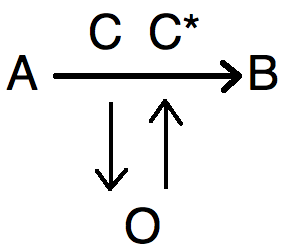
\includegraphics[width=3cm]{Simmons.png} 
\end{center}

Il y a 2 stratégies pour l'observateur O :\\

\begin{itemize}
\item \textbf{Imposture} (Impersonation) : O n'observe pas de transmission mais essaie de faire accepter $C^*$. (Réussite de probabilité $P_I$).
\item \textbf{Substitution} : O observe et substitue $C*\neq C$ 
(probabilité $P_S$).
\end{itemize}

	La probabilité de "tromperie" (deception) est $P_T= max(P_S$, $P_I)$.

\bigskip
	
\textit{exemple:} Il s'agit de chiffrer un ensemble de messages courts. $M=\{0$, $1\}$.

\bigskip

\textbf{I.}
\begin{center}
$\begin{array}{c|cc}
_K \ ^M & 0 & 1 \\
\hline
00 & 00 & 11 \\
01 & 01 & 10 \\
10 & 10 & 01 \\
11 & 11 & 00 \\
\end{array}$
\end{center}

$\bullet$ Confidentialité ?

\bigskip

$P(M=0\ \vert \ C=00) = \displaystyle\frac{P(M=0,\ C=00)}{P(C=00)}$\\
\hspace*{4,3cm}$=\displaystyle\frac{P(M=0,\ K=00)}{P(M=0,\ K=00) + P(M=1,\ K=11)}$\\
or K et M sont indépendantes donc \\
\hspace*{4,3cm}$=\displaystyle\frac{P(M=0)P(K=00)}{P(M=0)(1/4)+P(M=1)(1/4)}$\\
\hspace*{4,3cm}$=\displaystyle\frac{P(M=0)(1/4)}{1/4}$\\
\hspace*{4,3cm}$=P(M=0)$.\\

Le résultat est le même pour les autres calculs. La confidentialité est donc parfaite. Cependant, l'observateur peut substituer : $C=00 \rightarrow C^*=11$, il n'y a aucune authenticité, $P_S=1$.

\medskip

On observe par ailleurs, $P_I = \frac{1}{4}+\frac{1}{4}=\frac{1}{2}$.

\bigskip

\textbf{II.} On peut faire mieux que le premier cas.
\begin{center}
$\begin{array}{c|cc}
_K \ ^M & 0 & 1 \\
\hline
00 & 00 & 10 \\
01 & 01 & 00 \\
10 & 11 & 01 \\
11 & 10 & 11 \\
\end{array}$
\end{center}

$\bullet$ Confidentialité parfaite car le cas $P(M=0\ \vert \ C=00) =P(M=0)$ se généralise.\\

$P_I=\frac{1}{2}$.\\

On trouve $P_S=max(P(M=0)$, $P(M=1))$. Cette quantité peut être supérieure $1/2$ et même être proche de $1$. Peut-on faire mieux~?

\textbf{III.} 
\begin{center}
$\begin{array}{c|cc}
_K \ ^M & 0 & 1 \\
\hline
00 & 00 & 10 \\
01 & 01 & 11 \\
10 & 00 & 11 \\
11 & 01 & 10 \\
\end{array}$
\end{center}

$\bullet$ Confidentialité nulle.\\

$$P(K=00\ \vert \ C=00) = P(K=10\ \vert \ C=00) = \frac{1}{2} = P_S.$$

On a fait mieux que dans le cas précédent, mais pour descendre la probabilité de tromperie $1/2$ il a fallu sacrifier la confidentialité.

\bigskip

\underline{Remarque III:} $C=(M$, $\mathcal{S}(M,K))$, où $\mathcal{S}$ est une signature numérique.

\section{Sécurité Calculatoire (chiffres par flot, générateurs pseudo-aléatoires)}
\begin{itemize}
\item Taille des clés (comment l'engendrer ?)
\item Partage des clés ?
\end{itemize}

\bigskip
Idée simple : "Dégrader" le One-time pad en remplaçant $K_1,...,K_n$ par une suite pseudo-aléatoire $S_1,...,S_n,...$ engendrée par une clé secrète courte aléatoire.

\bigskip

\textit{exemple : }$s_1,...,s_n$ suite de bits $\{0,1\}$.\\
$s_i=f(s_{i-1}, s_{i-2},...,s_{i-m})$ dépend des $m$ bits précédents $f$ partiellement connue $s_0,...,s_{m-1}$, partie secrète.

\bigskip

\textit{exemple : }Générateur linéaire\\
$s_i=s_{i-1}h_{m-1}+s_i h_{m-2}+ ... + s_{i-m}h_0 \ (mod \ 2)$,\\
clé : $h_0,...,h_{m-1}, \ s_0,...,s_{m-1}$.\\
$c_i=M_i+s_i$ avec $s$ suite chiffrante.

%%%%%%%%%%%%%%%%%%%%%%%%%%%%%%%%%%%%%%%%%%%%%%%%%%%%%%%%%
%             		  Cyril BESLAY                      %
%%%%%%%%%%%%%%%%%%%%%%%%%%%%%%%%%%%%%%%%%%%%%%%%%%%%%%%%%
\subsection{Chiffre par flot( Stream Cipher)}

\begin{displaymath}
m = m_1 ...m_n
\end{displaymath}
\begin{displaymath}
\frac{+ "k" = S_1 ...S_n}{C_1 ... C_n }
\end{displaymath}

$s = s_1 ... s_n$ suite chiffrante Pseudo-aléatoire

$s = f(K)$\hspace{1cm} K clé courte

\hspace{2.8cm}$ K \in \{0,1\}^m$  $(=\{0,1\}^{128})$

Sécurité \underline{calculatoire} ($\neq$ inconditionnelle)\\

Types d'attaques
\begin{itemize}
\item Texte chiffré seul
\item Texte clair et chiffrés connus (ou partiellement)
\item Texte clair \underline{choisi}
\end{itemize}

\paragraph{Remarque :}
	Pour le chiffrement par flot, les attaques "Clair choisi" et "Clair connu" sont équivalentes.
	
	Le problème de la cryptanalyse, c'est de trouver la clé K  partir d'un certain nombre de symboles de la suite chiffrée $(s_1 ... s_n)$ ou encore  partir de $s_1..s_n$, trouver $s_{n+1},s_{n+2},...$. 
	
	De nos jours, on se place plutôt dans les 2 derniers cas plutôt que dans le cas de l'attaque par texte chiffré seul qui est trop restrictive.

\paragraph{Problème 1}
	Réaliser un générateur nombres pseudo-aléatoires
	$S_1...S_n...$ imprévisible
	
	\begin{displaymath}
	s_{n+1}=f_k(s_{n},s_{n+1},...s_{n-m+1})
	\end{displaymath}
	m "mémoire" du générateur
	\begin{displaymath}
	(s_{n+m},s_{n+m+1},...,s_{n+1})=F(s_{n},s_{n+1},...s_{n-m+1})
	\end{displaymath}
	
\paragraph{"Bonnes propriétés statistiques"}

	Remarque:
	
	$(S_i)$ est périodique
	
	au plus $2^m$ "états" du générateur
	
	$m-uples (S_n ...S_{n-m+\&})$
	
	Période max =$2^m$.
	
\paragraph{Question}
Que se passe t'il si la fonction $f$ est choisi aléatoire?

La suite ne peut être choisie aléatoirement mais le générateur oui.

\begin{displaymath}
f: \{0,1\}^m \mapsto \{0,1\}.
\end{displaymath}

Si on choisit le générateur aléatoirement (la fonction f), on s'attend  une période maxi nettement plus petite, elle sera en racine de $2^m$.

\subsubsection{Exemple: Von Neumann}
	Premier  vouloir utiliser des générateurs pseudo-aléatoires.(1946)
	
	Il marche de la manière suivante:
	\begin{displaymath}
	f:\{0,1\}^m \mapsto \{0,1\} \leftrightarrow F\{0,1\}^m \mapsto \{0,1\}^m
	\end{displaymath}
	\begin{displaymath}
	F:\{0, 99999\} \mapsto \{0,99999\}
	\end{displaymath}
	\begin{displaymath}
	x \mapsto x^2
	\end{displaymath}
	l'entier représenté par les 5 chiffres du milieu
	
	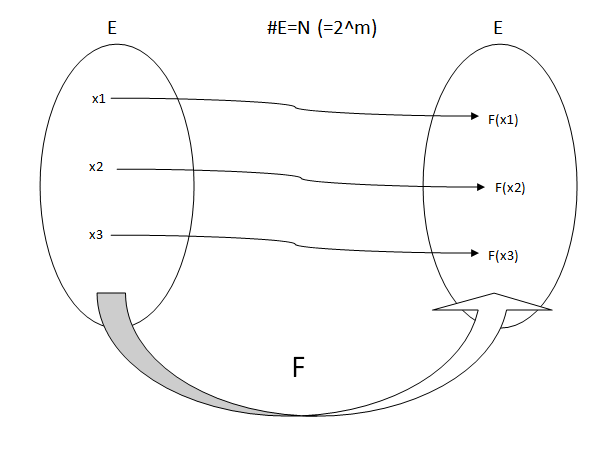
\includegraphics[width=14cm]{schema1.png} 
	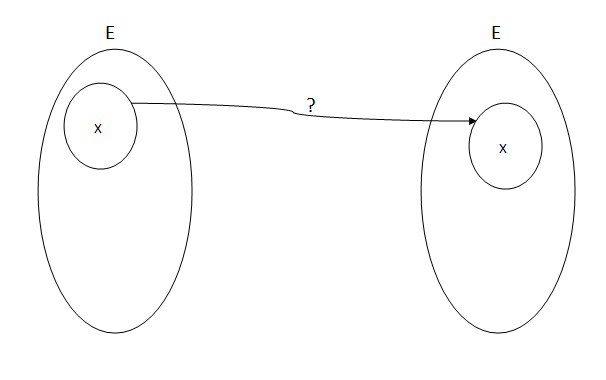
\includegraphics[width=14cm]{schema2.png} 
	\begin{displaymath}
	Probabilité \mapsto (\forall i, F(x_i) \not\in X_i) = \prod^{|X|}_{i=1} (1-\frac{|X_i|}{N})
	\end{displaymath}
	\begin{displaymath}
	\leq (1-\frac{|X|}{2N}) \simeq 1 - \frac{|X|^2}{4N}
	\end{displaymath}
	Problème quand $|X| \simeq \sqrt{N}$
	
	\paragraph{Problème 2}
	
	
$f:\{0,1\}^m \mapsto \{0,1\}$
	
$\# f = 2^{2^m}$
	
	

	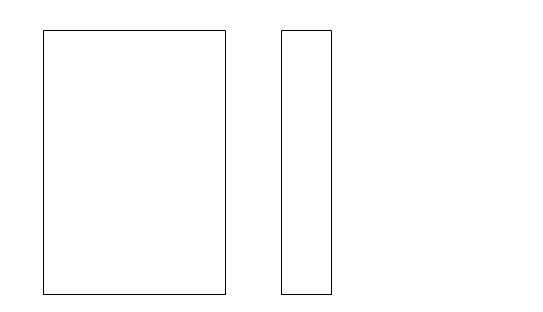
\includegraphics[width=14cm]{schema3.png} 


	\subsection{Cas des générateurs linéaires.}
	
	\begin{displaymath}
	S_i=S_{i-1}h_{m-1} + S_{i-2}h_{m-2} + ... + S_{i-m}h_{0} \pmod{2}
	\end{displaymath}
	
	\paragraph{Définition}
	\begin{displaymath}
	h(X)=X^m + h_{m-1}X^{m-1} + ... + h_1X + h_0 \in \mathbb{F}_2[X]
	\end{displaymath}
	Polynôme de réfraction de $s=(s_i)$
	
	LFSR (Linear Feedback Shift Register) Séquence
	
	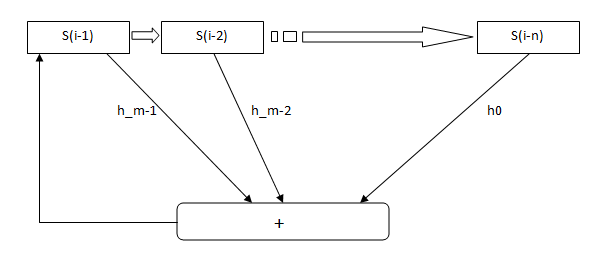
\includegraphics[width=16cm]{schema4.png} 
	
	\paragraph{Théorème}
		Si h(X) est :
		\begin{itemize}
		\item 1) irréductible
		\item 2) primitif
		\end{itemize}
		Alors période (s) $ = 2^m - 1$
	
	\paragraph{Primitif : }
		X d'ordre $\frac{2^m - 1}{e}$ dans $\mathbb{F}_2 [X]/h(X)$
		
		Plus petit entier e tel que
		$X^e - 1$ multiple de $h(X)$.
		
	Nous avons de bonnes propriétés statistiques.
	
	\underline{Mais} suites \underline{très} prévisibles.
	
	car $2m$ symboles consécutifs de la suite $(S_i)$ permettent de trouver les $h_i$ coefficients du générateur.
	\begin{displaymath}
\begin{tabular}{|c|c|c|}
  \hline
  $h_0$ & $S_0 ... S_{m-1}$ & $S_m ... S_{2m-1}$\\
  $h_1$ & $S_1 ... S_m$ & $S_{m+1} ...S_{2m-1}$ \\ 
  $h_2$ & $S_2 ... S_{m+1}$ & $S_{m+2}...S_{2m-1}$\\
  & $... ... ... ... ...$&\\ \hline
  & $S_m ... S_{2m-1}$&\\ \hline
\end{tabular}
		\end{displaymath}

	\begin{displaymath}
	h_0 S_0 + ... + h_{m-1} S_{m-1} = S_m
	\end{displaymath}
	\begin{displaymath}
	h_1 S_1 + ... + h_{m-1} S_{m-1} = S_{m+1}
	\end{displaymath}
	\begin{displaymath}
	... ... ... ...
	\end{displaymath}
	
	m relations , m inconnues
	
	\paragraph{Définition}
	Notion de complexité linéaire d'une suite
	
	Prenons une suite $(S_i)$ périodique quelconque.
	
	On appelle \underline{complexité linéaire} de $S$, la mémoire minimale d'un générateur linéaire qui engendre $S$. $\lambda (S)$ : la taille de la plus petite récurrence linéaire qui engendre $S$. 
	\\
	
	Remarque : $S_{i + \pi} = S_i)$ avec $\pi$ la période de la suite $S$ est une récurrence linéaire qui engendre $S$.
	
	Pour illustrer ce que l'on vient de dire, on veut (pour la cryptologie) un grand  $\lambda (S)$. $\leq2^{50}$.	
	
\bigskip
	
%%%%%%%%%%%%%%%%%%%%%%%%%%%%%%%%%%%%%%%%%%%%%%%%%%%%%%%%%
%             		Lionel RIVIERE                      %
%%%%%%%%%%%%%%%%%%%%%%%%%%%%%%%%%%%%%%%%%%%%%%%%%%%%%%%%%
\begin{center}
$\begin{array}{rccccccccc} 
      M & = & m_1 & . & . & . & m_n & . & . & .\\
+\;\; S & = & s_1 & . & . & . & s_n & . & . & .\\
\hline
      C & = & c_1 & . & . & . & c_n & . & . & .\\
\end{array}$
\end{center}	

$S_i=f(x_i^1,...,x_i^n)$.\\
Exemple : Geffe.\\

$\lambda(S)$ $(c_i=c_i+\pi)$\\

Stratégie de combinaison de LFSR\\
--------Schéma-----------\\


Exemple de Geffe\\
--------Schéma-----------\\

\medskip
\textbf{Théorème :} s,t deux suites périodiques.\\
\hspace*{2cm}$\bullet\ \lambda(s+t) \leq \lambda(s)+\lambda(t)$\\
\hspace*{2cm}$\bullet\ \lambda(st) \leq \lambda(s)\lambda(t)$\\

\textbf{Preuve :} s engendré par récurrence linéaire, mémoire m\\
$\circledast\ s_i=s_{i-1}h_{m-1}+...+s_{i-m}h_0$	\hspace*{1cm} avec $m=\lambda(s)$\\
L'ensemble des solutions E de $\circledast$ est stable par addition, donc c'est un espace vectoriel sur $\mathds{F}_2 = (\{0,1\},+,x)$. Toute solution s de $\circledast$ s'écrit : \\
$$s=\alpha_1e^1+\alpha_2e^2+...+\alpha_ke^k$$ 
où $(e_1,...,e_k) $ est une base de E, \\
$\alpha_i \in \mathds{F}_2$ écriture unique,\\
k=m ($dim(E)=n$ car espace vectoriel de dimension k contient $2^k$ éléments et on a $2^m$ suites possibles).\\

\medskip

$$t=\beta_1f_1+...+\beta_{m^{'}}f_{m^{'}}$$
où $m^{'}=\lambda(t)$\\
$s+t$ est dans l'espace engendré par $(e_1,...,e_m,f_1,...,f_{m^{'}})$, $dim(E+F)\leq m=m^{'}$. 
 $\square$
 
\medskip
 
$\lambda(s+t)$ dimension de l'espace des décalés de $s+t$

$\left\lbrace
\begin{array}{ll}
	s_0\ s_1\ s_2\ .\ .\ .\\
	s_1\ s_2\ s_3\ .\ .\ .\\
	. \\
	. \\
	. \\
	s_m\ s_{m+1}\ s_{m+2}\\
\end{array}
\right.$
 
$(s+t)_{i+d} = s_{i+d}+t_{i+d}$ \\
\begin{eqnarray*}
st &=&  (\alpha_1  e_1 +...+ \alpha_m e_m) ( \beta_1 f_1 +...+ \beta_{m_{^{'}}} f_{m^{'}}) \\
   &=& \sum_{i,j}\ \alpha_i \beta_j e_i f_i \\ 
\end{eqnarray*}

$(e_1 f_1 ,..., e_1 f_{m^{'}}, e_2 f_1, ..., e_2 f_{m^{'}}, ..., e_m f_1, ..., e_m f_{m^{'}})$ engendre $(s_{i+d} t_{i+d}) = ((st)_{i+d}). \square $

\medskip
\hspace*{-0,6cm}$\lambda(a) = \lambda(b) = \lambda(c) = 128$\\
$\lambda(s) \leq \lambda(a) + 2\times 128^2$\\

\medskip
Autre problème : Corrélation entre $s_i$ et $a_i$.
\begin{itemize}
\item si $b_i = 0$, $s_i = a_i$
\item si $b_i = 1$, $s_i = c_i = \alpha_i$ indépendant de $a_i$ une fois sur deux.
\item si $s_i = a_i$, 3 fois sur 4.
\end{itemize}

$s=f(x_1,...,x_n)$ doit résister aux corrélations s indépendantes de $x_i$.\\

\section{Chiffres par blocs}
\begin{eqnarray*}
f\ :\ \{0,1\}^m \times \{0,1\}^k &\longrightarrow & \{0,1\}^m \\
(M, K) & \longmapsto & C \\
\end{eqnarray*}

\subsubsection{Suggestion de Shannon}
\begin{center}
Diffusion \hspace*{5cm} Confusion\\
\end{center}

Alterner des substitutions et des "transpositions" (ou applications linéaires).\\

m=64,128\\
--------Schéma-----------\\

IBM : Lucifer \\
m=k=128\\
$S_0, S_1 \ \ {0,1}^8 \longrightarrow {0,1}^8$.\\

\subsubsection{Idée de Feistel}

Idée de Feistel\\
--------Schéma-----------\\

%%%%%%%%%%%%%%%%%%%%%%%%%%%%%%%%%%%%%%%%%%%%%%%%%%%%%%%%%
%             		  Cyril BESLAY                      %
%%%%%%%%%%%%%%%%%%%%%%%%%%%%%%%%%%%%%%%%%%%%%%%%%%%%%%%%%

\subsection{DES}

DES qui est restée la principale norme de chiffrement (1973-1998), a nécessité des efforts importants en cryptanalyse. Rendu complètement publique, beaucoup on essayé d'en montrer les faiblesses. Les attaques contre le DES donne la célébrité assurée.

Les espaces de clé n'étaient pas très grand $K \in \{0,1\}^{56}$. Cet espace était TOUT juste trop (donc beaucoup de controverse). 2 attaques ont été trouvées. Ce sont des attaques susceptibles de fonctionner sur tout les modèles.\\

\begin{itemize}
\item La cryptanalyse différentielle (1991, Shamir, Biham)

C'est une attaque  clair choisi qui ne fonctionne pas bien avec le système DES. Il s'agit d'une attaque statistique.\\

\item La cryptanalyse linaire (1994, Matsumuto)

C'est une attaque  clair connu.

Idée : essayer de trouver une relation linaire qui relit les bits du cryptogramme et les bits de la clé. Est ce que l'on peut trouver une relation du type $M_1+M_3+M_7+...M_{59}+K_2+...+K_{32}+K_{35}+C_3+C_{24}+...+C_{61}=0$

$M_1$ premier bit du message en clair

$K_2$ bit de la cl

$C_3$ bit du cryptogramme

Il y aurai 1 bit qui se calcul en fonction des autres. A chaque fois, on divise par 2 l'espace des clés. Dis comme ça, c'est utopique car il n'existe pas de relation normalement, mais on peut espérer qu'il y ai de telles relations.

La probabilité d'avoir de telles relations est $\frac{1}{2}-\varepsilon$ ou $\frac{1}{2}+\varepsilon$ et existe \underline{forcement} pour un $\varepsilon > 0$.\\

$C_1=f(M,K)$ non linaire, il y a un vrai espoir de trouver une relation

Si jamais on trouve une telle relation, au lieu d'avoir besoin d'un couple clair chiffré, il en faut plusieurs, par exemple, si cette relation est satisfaite avec une probabilité de $\varepsilon$, il faut regarder n couples $M,C$, et calculer $M_1+M_3+M_7+...M_{59}+K_2+...+K_{32}+K_{35}+C_3+C_{24}+...+C_{61}=0$, de regarder combien de fois ça vaut 0, combien de fois a vaut 1, si on trouve une majorité de 0, ça veut dire que la somme des bits de cl $K$ valent 0, donc $K_2+...+K_{32}+K_{35}$.\\

La question primordiale: Combien de couple (clair, chiffré) faut t'il?\\

Quel est l'ordre de grandeur de n pour très sure du résultat?\\

Hypothèse: Valeurs indépendantes de la somme $\sum M_i + C_i$

Pour un n assez grand, la loi des grand nombre, on doit trouver $n(\frac{1}{2} - \varepsilon)$ mais en pratique, il y aura des fluctuations dont l'ordre de grandeur est: $O(\sqrt{n})$

Il faut que le $\sqrt{n} \leq n \varepsilon$

ou encore $\sqrt{n} \geq \frac{1}{2}$

$n \geq \frac{1}{\varepsilon^2}$\\

Avec le DES on a un $\varepsilon$ qui vaut environ $2^{-21}$ avec un $n \approx 2^{43}$
\end{itemize}

\subsubsection{Successeurs du DES}

\subparagraph{Triple DES}
\begin{itemize}
\item $K \in  \{0,1\}^{3*56} = \{0,1\}^{168}$.

$f_k(M) = DES_{K_3}(DES_{K_2}(DES_{K_1}(M)))$

\item $E_{K_1}(D_{K2}(E_{K_1}(M))), K=(K_1,K_2)\in \{0,1\}^{112}$

$K_1=K_2 \Rightarrow$ DES simple

\end{itemize}
\subparagraph{Chiffrement double}

\begin{itemize}
\item $ M \longmapsto f_{K_2}(f_{K_1} (M)) =C $ on obtient un système de chiffrement a peine plus sure que le simple

Attaque "par le milieu

M,C clair-chiffré.

Admettons la table suivante

\begin{tabular}{|c|c|c|}
\hline $f_K(M)$ &  & $f_K^{-1}(C)$ \\ 
\hline \vdots &  & \vdots \\ 
\hline \vdots &  & \vdots \\ 
\hline \vdots &  & \vdots \\ 
\hline $K \in \mathcal{K}$ &  & $K \in \mathcal{K}$ \\
\hline 
\end{tabular} 

Regarder dans les 2 tableaux quel est la valeur commune

\end{itemize}

\subsection{AES (Advanced Encryption Sandard)}

crée par Rijndael

$M_1 K \in \{0,1\}^{128}$
\\ 

$M$

$\bigoplus \longleftarrow K_0 = K$

$Ronde 1 $

$\bigoplus \longleftarrow K_1 = K$

$Ronde 2$

$\bigoplus \longleftarrow K_2 = K$

$\ \ \vdots$

$Ronde 10$

$\bigoplus \longleftarrow K_{10} = K$

$ C $\\

Ronde i : $M_i \longrightarrow  $ substitution $ \longrightarrow $ application linaire

Substitution : Une application $\{0,1\}^8 \rightarrow \{0,1\}^8$

$M_i$ 16 octets

Application algébrique : $\mathbb{F}_2 [X] / (X^8+X^4+X^3+X+1) \rightarrow \mathbb{F}_2 [X] / ( \ \ )$

$\sigma : P \mapsto P^{-1}$

$\ \ \ \ 0 \mapsto 0$

$\sigma$ coïncide (conjecture) le moins souvent avec application affine.



$S:\{0,1\}^8 \longrightarrow \{0,1\}8$

$\ \ \ x \longmapsto A \sigma (x) +b$

\begin{displaymath}
A = 
\begin{pmatrix}
1 & 0 & 0  & 0 & 1 & 1 & 1 & 1 \\ 
1 & 1 & 0 & 0 & 0 & 1 & 1 & 1 \\ 
1 & 1 & 1  & 0 & 0 & 0 & 1 & 1 \\ 
\vdots & \vdots & \vdots & \vdots & \vdots & \vdots & \vdots & 
\end{pmatrix} 
\longrightarrow b = 
\begin{pmatrix}
1 \\ 
1 \\ 
0 \\ 
0 \\ 
0 \\ 
1 \\ 
1 \\ 
0
\end{pmatrix} .
\end{displaymath}

Application linéaire.



\begin{displaymath}
\begin{pmatrix}
a_{11} & a_{12} & a_{13} & a_{14} \\ 
 &  &  &  \\ 
 &  &  &  \\ 
a_{41} &  &  & a_{44}
\end{pmatrix} 
\longrightarrow
\begin{pmatrix}
a_{11} & a_{12} & a_{13} & a_{14} \\ 
a_{22} & a_{23} & a_{24} & a_{21} \\ 
a_{33} & a_{34} & a_{31} & a_{32} \\ 
a_{44} & a_{41} & a_{42} & a_{43}
\end{pmatrix} 
\end{displaymath}

2 applications successives:

\begin{itemize}
\item 1) Shift Rows
\item 2) Mixcolumns
\end{itemize} 

\begin{displaymath}
\begin{pmatrix}
a \\ 
b \\ 
c \\ 
d
\end{pmatrix} 
\longleftrightarrow
a(X) = a+ bX + cX^2 + dX^3
\end{displaymath}

$a(X) \rightarrow a(X) x(X) mod (X^4 +1)$

$c(X) = (03)X^3 + X^2 + X + (02)$

$03 = [00000011] = (x+1) mod (x^8+x^4+x^3+1$

Ronde 10 : pas de Mixcolumns.\\

Clé $K_i$ ?

$K=K_0$

//SCHEMA//

$w(i)=w(i-1)+w(i-4)$ si $i\neq 0 \bmod{4}$

$w(i)=Ti(w(i-1))+w(i-4)$ si $i=0 \bmod{4}$
\\

Avec Ti: \begin{displaymath}
\begin{pmatrix}
a\\
b\\
c\\
d\\
\end{pmatrix}
\mbox{-->}
\begin{pmatrix}
b\\
c\\
d\\
a\\
\end{pmatrix}
\mbox{-->}
\begin{bmatrix}
S(b)\\
S(c)\\
S(d)\\
S(a)\\
\end{bmatrix}
\mbox{-->}
\begin{bmatrix}
S(b)+e_i\\
S(c)\\
S(d)\\
S(a)\\
\end{bmatrix}
\end{displaymath}

$e_{i}=[00000010]^{(i-4)/4}$
\\

*Modes opératoires:

$f_k:\{0,1\}^N-->\{0,1\}^N$

$M_1,M_2,...,M_i,... -->f_k-->C_1,C_2,...,C_i,...$

Si on observe $C_i=C_j$, alors on en déduit $M_i=M_j$.\\

\begin{itemize}
\item{Mode ECB (electronic code book)}

Pb: dictionnaire de chiffrés\\

\item{Mode CBC (cipher block chaining)}

$C_j=f_k(M_j+C_{j-1}=$

$C_0=VI$ (= valeur aléatoire) --> communiqué en clair\\

\item{Mode CFB (cipher feedback)}

$C_j=M_j+f_k(C_{j-1})$\\

\item{Mode OFB (output feedback)}

$X_0=VI$ clair

$X_j=f_k(X_{j-1})$ et $C_j=M_j+X_j$

transforme le chiffre par blocs en chiffre par flot\\

\end{itemize}

\section{Fonctions sens unique (ou difficilement inversibles) one-way}

\subsection{Définition}

$f:(K,VI)\rightarrow\{0,1\}^n$\\

Fonctions bijectives:

f  "sens unique" s'il $\exists$ un algorithme efficace qui calcule $f(x)$ et s'il $\not\exists$ un algorithme efficace qui calcule $x$  partir de $f(x)$\\

$f:\{0,1\}^n\rightarrow \{0,1\}^n$

$E\rightarrow E$

$x\rightarrow f(x)$\\

\subsection{Protection des mots de passe}

$U\rightarrow m\rightarrow M$ avec $m\in \{m_0,m_1,...,m_k\}$

On stocke plutôt les $f(m_i)$.

La machine compare ensuite les $f(m_i)$ au $f(m)$ donné.

Pas d'accès possible si on ne sait pas inverser f.\\

Procédé de Lamport:

connexions  distance\\

$U \rightsquigarrow M$

$m_0$

$m_1=f(m_0)$ et $m_i=f(m_{i-1}) \rightarrow$ envoie $m_i$

U envoie $m_999$

M fait $m_1000=f(m_999)$

si $m_1000$ apparaît $\rightarrow$ accepte puis remplace $m_1000$ par $m_999$

U envoie $m_998$ etc

\subsection{Quelles fonctions peuvent être  sens unique?}

Fonction + dans $\mathbb{Z} /n\mathbb{Z} \rightarrow$ non (trop simple)

Fonction x dans $\mathbb{Z} /n\mathbb{Z} \rightarrow$ non (inversible)



Fonction  sens unique (one-way)

\begin{displaymath}
f:x \longmapsto f(x)
\end{displaymath}
\begin{displaymath}
\longleftarrow
\end{displaymath}

Candidat:

\begin{displaymath}
f: x \longmapsto \alpha ^ x mod (n)
\end{displaymath}

pas de $f^{-1}$ de même nature $\beta^{\alpha^x}$

\begin{displaymath}
y = \alpha^x mod (n)
\end{displaymath}

En général, le temps de calcul pour trouver x  partir de $y=\alpha^x mod (n)$ 

- Recherche exhaustive: $\sim$ n opérations dans $\mathbb{Z}/n\mathbb{Z}$ --> $m=2^{log n}$


Meilleurs algortithmes: $2^{c \sqrt{log n}}$ 
(sous-exp --> $2^{c(log n)^{\frac{1}{3}}}$)

\paragraph{Calculabilité de f}

Elévations au carré successives

\begin{displaymath}
x=\sum_{i\in I} 2^i
\end{displaymath}
\begin{displaymath}
\alpha ^x = \prod _{i \in I} \alpha ^{2^i}
\end{displaymath}
\begin{displaymath}
\alpha^{2^i} = ((\alpha ^2)^2)^{...2}
\end{displaymath}

\paragraph{Choix de f} i.e de $\alpha$ , n

Par exemple, pour que f soit une bijection 

\begin{displaymath}
\{0,1,2,...,n-2\} \longrightarrow^f \{1,2,...,n-1\}
\end{displaymath}
\begin{displaymath}
x \longmapsto \alpha^x mod(n)
\end{displaymath}

\subparagraph{Théorème (Elément primitif)}

Si n premier, $\exists$ $\alpha$ (primitif)
t.q f est une bijection:

\begin{itemize}
\item $1, \alpha, \alpha^ 2 , ... , \alpha ^{n-2}$ sont 2  2 $\neq$
\item ordre de $\alpha = n-1$
\end{itemize}

\subparagraph{Trouver n, $\alpha $ adéquats ?? (Théorème de Lucas)}

n est premier ssi $\exists \alpha $ t.q

\begin{itemize}
\item $\alpha^{n-1} = 1 mod(n)$
\item $\forall q (n-1)$, q premier, $\alpha^{\frac{n-1}{q}} \neq 1 mod(n)$
\end{itemize} 

\subparagraph{$\Rightarrow$}

si n premier . Th de l'element primitif

\subparagraph{$\Leftarrow$}

Si

\begin{displaymath}
\alpha ^{n-1}= 1mod(n), \alpha \in (\mathbb{Z}/n\mathbb{Z})^*
\end{displaymath}
 
Le nombre d'éléments dans le groupe x est $\varphi(n)$

\begin{displaymath}
\frac{\alpha^{\varphi(n)} = 1}{\alpha^{n-1} =1} \ \ \alpha^{pgcd(n-1,\varphi(n))} =1
\end{displaymath}

\begin{displaymath}
\varphi(n) = n-1   \bullet
\end{displaymath}

2 idées clés.
\begin{itemize}
\item n,$\alpha$ au hasard

\subparagraph{Justification}

Beaucoup de nombres premiers.

$\pi (n) \sim \frac{n}{ln n}$

Proba $ \simeq \frac{1}{ln n}$

\item imposer q : imposer les facteurs de $n-1$

Choisir $q_1 ....q_k$ premier

$n= 1 + q_1^{m_1} ... q_k^{m_k}$
\end{itemize}

\subparagraph{Concretement:} Pour fabriquer des nombres premiers de plus en plus grand.

\begin{displaymath}
Q=\{2,3,5, .....\}
\end{displaymath}

\begin{itemize}
\item 1)$q \simeq 2^{50}$
\item 2)$q \simeq 2^{100}, 2^{150},...$
\end{itemize}

Chercher simultamement $\alpha,n.$

Seule manière connue d'avoir $\alpha$ primitif mod (n)

\begin{displaymath}
x \longmapsto \alpha^x  mod (n).
\end{displaymath}

\begin{displaymath}
(\alpha^a)^b =(\alpha^b)^a.
\end{displaymath}

\paragraph{Protocole de Diffie-Hellman(1976)}

Résoudre le problème du partage des clés.

ATTENTION SHEMA DE ALICE ET BOB


A et B partagent $\alpha$ , p premier, $\alpha$ primitif mod p

(publie)

A choisi a secret, calcul $\alpha^a mod(p)$, le donne  B.

B choisi b secret, calcul $\alpha^b mod(p)$, le donne  A.

A et B conviennent de Partager

\begin{displaymath}
S=\alpha^ {ab} mod (p)
\end{displaymath}

\begin{displaymath}
A: (\alpha^b)^a = S mod (p)
\end{displaymath}

\begin{displaymath}
B: (\alpha^a)^b = S mod (p)
\end{displaymath}

\paragraph{Conclusion :}

Si le problème de DH est algoritmmiquement difficile, alors A et B savent partager un secret donc le protocole est efficace

\paragraph{Chiffrement}

Idée de clé "publique".

\begin{displaymath}
f_k : M \longmapsto C \longmapsto f_k^{-1} (C) = M
\end{displaymath}

$(f,f^{-1})$ un algorithme $\mathcal{A}$ pour calculer $f$ et un algorithme $\mathcal{B}$ pour calculer $f^{-1}$. 

\subparagraph{Idée:}

B garde $\mathcal{B}$ secret (destinataire) 

mais rend public $\mathcal{A}$ (calcul $f$)

\begin{displaymath}
A : \mathcal{A}(M) \longrightarrow^C B. \mathcal{B}(C) = M
\end{displaymath}

Pour cela il faut:

$f$  sens unique "avec trappe" (frapdoor) $\exists \mathcal{B}, \exists$ secret qui permet de calculer $f^{-1}$

\paragraph{Chiffrement El Gamal}

Publiques; $\alpha, p,$ et $P=\alpha^s mod(p)$

Secret: s

\subparagraph{Chiffrement:} $\alpha, p, P.$

A choisit k au hasard 

$C_1 = \alpha^k mod(p)$

$C=(C_1,C_2)$

$C_2 = MP^k$

\subparagraph{Déchiffrement:} s

\begin{displaymath}
P^k = \alpha^{sk} = (\alpha^k)^s = C^s_1
\end{displaymath}

\begin{displaymath}
M = C_2(C_1^ s)^{-1} mod(p)
\end{displaymath}


Il suffit d'un groupe commutatif G

\begin{displaymath}
x \longmapsto \alpha^x \ a \ sens \ unique.
\end{displaymath}

 
\end{document}